\newpage


\section{Przegląd metod detekcji}\label{sec:przeglad-rozwiazan}

\subsection{Rate Limiting}\label{subsec:rate-limiting}

Rate Limiting to technika kontrolująca tempo, w jakim klienci mogą wysyłać żądania do serwera API\@.
W tym celu zlicza się liczbę żądań w określonym oknie czasowym, a następnie ustala, czy ich częstotliwość nie przekracza maksymalnego dopuszczalnego progu~\cite{api-rate-limit-adoption}.

Rozwiązanie zazwyczaj polega na liczeniu czasu między każdym żądaniem z każdego adresu IP\@.
W przypadku, kiedy liczba żądań z danego adresu IP przekroczy ustalony limit w danym oknie czasowym, żądanie kończy się odpowiednim błędem.
Adres IP, w tym przypadku, służy jako identyfikator klienta~\cite{cloudflare-what-is-rate-limiting}.
Jednak, dopuszcza się również inne identyfikatory.

Brak rate limitingu API jest, według \emph{OWASP API Security Top 10}, uznawany za podatność.
W punkcie \emph{API4:2019 Lack of Resources \& Rate Limiting}, autorzy wskazują, że:\@
\begin{displayquote}[\citetitle*{owasp-api-security-top-10}~\cite{owasp-api-security-top-10}, tłum. własne]
    ``Żądania API zużywają zasoby takie jak sieć, CPU, pamięć i miejsce na dysku.
    Ilość zasobów potrzebnych do zaspokojenia żądania w dużej mierze zależy od danych wejściowych użytkownika i logiki biznesowej koncówki.
    Należy również wziąć pod uwagę fakt, że żądania od wielu klientów API konkurują o te same zasoby.
    API jest podatne na problemy, jeśli brakuje przynajmniej jednego z następujących limitów lub są one ustawione nieodpowiednio (np. zbyt niskie/wysokie):

    \begin{itemize}
        \item Limit czasu wykonania
        \item Maksymalna alokowalna pamięć
        \item Liczba deskryptorów plików
        \item Liczba procesów
        \item Rozmiar ładunku żądania (np. przesyłane pliki)
        \item Liczba żądań na klienta/zasób
        \item Liczba rekordów na stronę zwracanych w pojedynczej odpowiedzi na żądanie''
    \end{itemize}
\end{displayquote}

Rate Limiting stosuje się do ochrony ograniczonych zasobów, obrony przed atakami typu odmowa dostępu (ang. \emph{DoS, Denial of Service})
oraz blokowania aktywności botów generujących duże nadużycia API\@.

\newpage

\subsection{Reverse Proxy --- blokowanie oparte na regułach}\label{subsec:reverse-proxy}

Termin proxy, w dziedzinie sieci komputerowych, określa aplikacje serwerową, która działa jako pośrednik między klientem wysyłającym żądanie a serwerem docelowym.
Wyróżnia się dwa główne typy proxy: forward proxy i reverse proxy.
Oba te typy działają na brzegu sieci.
W uproszczeniu, pierwszy z nich pośredniczy między klientem a internetem, podczas gdy drugi zarządza ruchem przychodzącym z internetu do serwerów.
Uszczegóławiając, reverse proxy najczęściej znajduje się na brzegu sieci przed jednym lub wieloma serwerami.
Klient wysyła żądanie do serwera proxy, a ten je przechwytuje i przekazuje do serwerów docelowych~\cite{cloudflare-what-is-reverse-proxy}.
Działanie reverse proxy zostało przedstawione na \autoref{fig:reverse-proxy}.

\begin{figure}[H]
    \centering
    \captionsetup{width=.7\linewidth}
    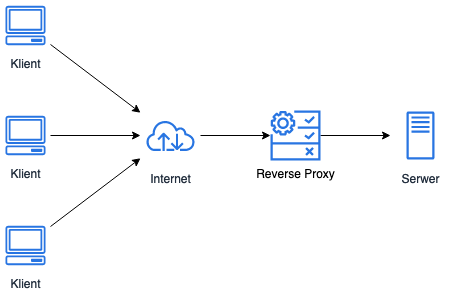
\includegraphics[width=0.8\textwidth]{img/reverse-proxy}
    \caption{Uproszczony schemat działania reverse proxy}
    \label{fig:reverse-proxy}
\end{figure}

Serwery reverse proxy znajdują swoje zastosowanie w detekcji web scrapingu ze względu na swoją zdolność do filtrowania ruchu przychodzącego.
Jak wskazano w \autoref{subsec:scraper}, ruch sieciowy generowany przed scrapery może oznaczać się charakterystycznymi cechami.
Na podstawie każdego z punktów w wspomnianym \autoref{subsec:scraper} można stworzyć regułę blokującą web scraping.

\newpage

\subsection{Browser Fingerprinting}\label{subsec:browser-fingerprinting}

\todo{Browser Fingerprinting}

\newpage

\subsection{Bot Detection as a Service}

\todo{Bot Detection as a Service}
